\section{Geometria Trifocal: detalhamento da abordagem de Nistér e Schaffalitzky.}\label{sec.nister}

Para abordar um problema trifocal, primeiro \cite{2503343} desenvolvem uma abordagem num sistema bifocal para determinação da rotação e da translação (supondo qua a calibração já seja conhecida) da segunda câmera em relação à primeira, utilizando duas imagens com quatro pontos correspondentes. Eles demonstram que os epipolos de cada imagem estão restritos a se alojarem numa curva de grau 10, a chamada curva décica, bem como desenvolvem um método para a obtenção dessa curva. De posse dos epipolos, definem a geometria epipolar, resgatam a segunda câmera em relação à primeira e fazem a reconstrução 3D dos quatro pontos. Com os pontos em 3D e a terceira imagem, resgatam a terceira câmera consistente com a estrutura 3D definida pelas duas primeiras câmeras. Utilizam essa teoria para desenvolver o que chamaram de solução mais eficiente para época (2006), o notório desafio de estabelecer as poses das câmeras num sistema com três imagens e quatro pontos. O artigo possui vários teoremas e alguns deles são interessantes em termos de pesquisas em geometria projetiva. Por isso, vamos reproduzir o enunciado dos teoremas e abriremos subseções explicando conceitos e definições que são importantes ao entendimento dos teoremas. Depois de realizadas essas explicações será fornecida a demonstração de alguns teoremas, os quais as demonstrações não se encontram no artigo.

\begin{figure}[!htb]
\centering
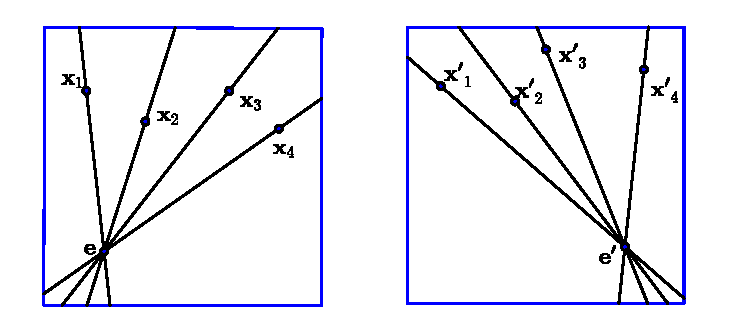
\includegraphics[scale=1]{retas-epipolares}
\caption{\textit{Feixe de retas passando pelo epipolo em cada imagem, relacionadas duas a duas por uma homografia.}}
\label{retas-epipolares}
\end{figure}

\subsection{O teorema 1}\label{sec.homografia-reta-epipolar} 


Uma das primeiras afirmações do artigo é que as retas epipolares numa  imagem estão homograficamente relacionadas com as retas epipolares na segunda imagem. Dados $n$ correspondências de pontos em duas imagens, o teorema trata da \textit{restrição epipolar} \citep{faugeras93three}. Ou seja, temos uma homografia 1D que relaciona o feixe de retas através ${\bf e}$ com o feixe de retas através ${\bf e'}$ chamada \textit{homografia da reta epipolar}. Podemos visualizar essa situação na figura \ref{retas-epipolares}.

\begin{teorema}
As $n$ retas passando pelos pontos $\e$ e $\x_i$ na primeira imagem estão homograficamente relacionadas com as $n$ retas passando por $\e'$ e $\x'_i$ na segunda imagem.
\end{teorema}

\begin{proof}
Segundo \cite{Hartley2004}, o feixe de retas epipolares em cada imagem estão perspectivamente relacionados através do centro de projeção $Q$ na reta base, conforme a figura \ref{fig.retas-epi-hartley}.

\begin{figure}[!htb]
\centering
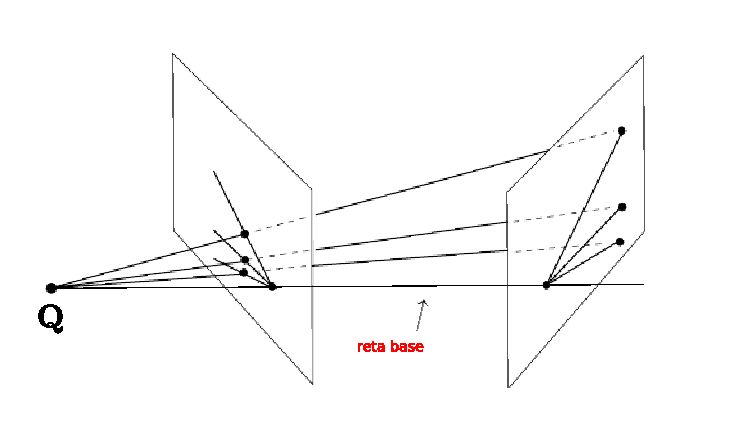
\includegraphics[scale=1]{retas-epipolares-hartley}
\caption{\textit{Retas epipolares com perspectiva centrada em $Q$ na reta base.}}
\label{fig.retas-epi-hartley}
\end{figure}


Suponha que $\lightrgb$ e $\lightrgb'$ sejam duas retas epipolares correspondentes, e ${\bf m}$ é uma reta qualquer que não passa pelo epipolo $\e$. O produto vetorial 

\begin{equation}
{\bf m}\times\lightrgb=\x\qquad\text{ou}\qquad\,[{\bf m}]_\times\,\lightrgb=\x,
\end{equation}
nos fornece o ponto $\x$ de interseção entre essas retas. Pela subseção \ref{sec.matriz-F} temos que

\begin{equation*}
\lightrgb'=F\,\x,
\end{equation*} 
assim, $\lightrgb$ está relacionada a $\lightrgb'$ através da equação 

\begin{equation*}
\lightrgb'=F\,[{\bf m}]_\times\,\lightrgb.
\end{equation*}


Uma boa escolha para ${\bf m}$ é a reta $\e$, já que

\begin{equation*}
{\bf m}^\top\e=\e^\top\e\neq0,
\end{equation*}
então $\e$ é uma reta que não passa pelo epipolo $\e$ como desejado. Assim, a homografia da reta epipolar pode ser escrita como 

\begin{equation*}
\lightrgb'=F\,[\e]_\times\,\lightrgb.
\end{equation*}
O argumento é análogo para o mapeamento da segunda imagem para a primeira,

\begin{equation*}
\lightrgb=F^\top [\e']_\times\,\lightrgb'.
\end{equation*}\\


\end{proof}


\subsubsection{A homografia da reta epipolar} 


Outra forma de pensar sobre essa homografia é realizando uma translação de forma que os epipolos estejam na origem do plano de cada imagem, e com as retas epipolares passando pelo epipolo, cada reta pode ser parametrizada através do ângulo que ela forma com o eixo das abscissas, denominados $\alpha_1$ e $\alpha_2$ na primeira e segunda imagens respectivamente.
A homografia da reta epipolar pode ser representada pela equação de uma hipérbole alinhada aos eixos perpendiculares, conforme descrito em \cite{Fabbri:Kimia:CVPR10},
\begin{equation}\label{eq.hiperbole}
a\,x\,y+b\,x+c\,y+d=0 \qquad \text{ou} \qquad y=\frac{-b\,x-d}{a\,x+c},
\end{equation} 
onde $x=tan\,\alpha_1$ e $y=tan\,\alpha_2$. 

Vemos na figura \ref{fig.reta-epipolar} que cada reta epipolar fica definida por um ponto no eixo da tangente, $(1,tan\,\alpha_1)$ na primeira imagem e $(1,tan\,\alpha_2)$ na segunda, onde consideramos o círculo trigonométrico de raio $1$. Usando esses pontos, a equação da hipérbole pode ser escrita na forma

\begin{equation}\label{eq.homo-reta-epi}
(1\,,\,tan\,\alpha_1)
\overbrace{
\begin{bmatrix}
d&c\\
b&a
\end{bmatrix}
}^{H}
\begin{pmatrix}
1\\
tan\,\alpha_2
\end{pmatrix}
=0,
\end{equation}
sendo 
$\begin{bmatrix}d&c\\b&a\end{bmatrix}$ a homografia procurada.

O problema é que a equação \ref{eq.homo-reta-epi} não está definida para retas epipolares verticais, pois utilizamos a tangente, e uma saída é parametrizar cada reta através da própria definição de tangente, pois assim temos uma representação isotrópica para as retas:

\begin{equation}\label{eq.tan.alpha1-2}
x=tan\,\alpha_1=\frac{sen\,\alpha_1 }{cos\,\alpha_1} \qquad \text{e} \qquad y=tan\,\alpha_2=\frac{sen\,\alpha_2}{cos\,\alpha_2}.
\end{equation} 

Desta forma, substituindo \ref{eq.tan.alpha1-2} em \ref{eq.hiperbole} e multiplicando por $cos\,\alpha_1\,cos\,\alpha_2$ temos

\begin{equation*}
a\,sen\,\alpha_1\,sen\,\alpha_2+b\,sen\,\alpha_1\,cos\,\alpha_2+c\,cos\,\alpha_1\,sen\,\alpha_2+d\,cos\,\alpha_1\,cos\,\alpha_2=0.
\end{equation*}

\begin{figure}[!htb]
\centering
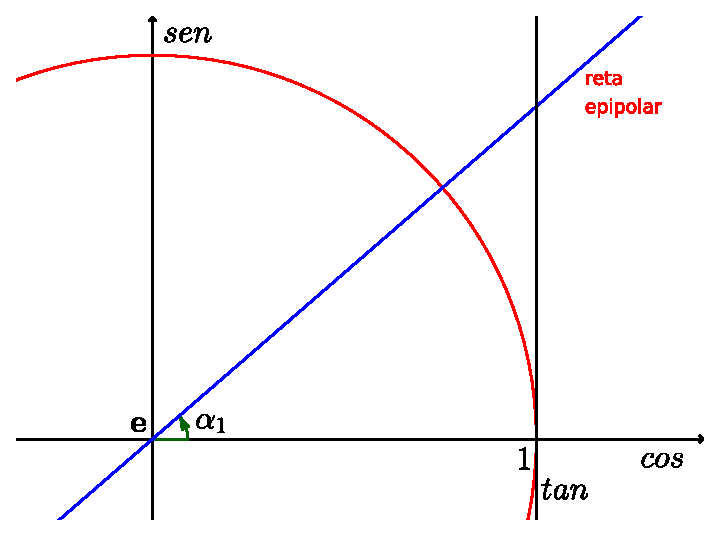
\includegraphics[scale=.8]{reta-epipolar-alpha1}
\caption{\textit{Plano da imagem centrado em ${\bf e}$ com a reta epipolar parametrizada por $\alpha_1$.}}
\label{fig.reta-epipolar}
\end{figure}

Com essa conversão, deixamos de parametrizar as retas epipolares pelo eixo das tangentes e passamos a parametrizar pelo círculo trigonométrico. Aqui temos um argumento para contagem dos graus de liberdade para fixarmos a relação entre retas epipolares, pois devemos determinar os dois epipolos (duas variáveis cada totalizando quatro graus de liberdade), e mais a matriz que representa a homografia (quatro variáveis mas apenas três graus de liberdade utilizando uma variável para fixar a escala). Portanto, precisamos de no mínimo sete restrições para determinarmos a relação entre duas imagens na geometria epipolar. 

Na nossa abordagem, consideramos o círculo trigonométrico com raio $1$ mas, segundo \cite{Fabbri:Kimia:CVPR10}, podemos estipular raios arbitrários $r_1$ e $r_2$ em cada uma das imagens que ajuda a garantir estabilidade numérica para a determinação dos coeficientes. Assim, obtemos a equação:

\begin{equation*}
a\,r_1\,sen\,\alpha_1\,r_2\,sen\,\alpha_2+b\,r_1\,sen\,\alpha_1\,r_2\,cos\,\alpha_2+c\,r_1\,cos\,\alpha_1\,r_2\,sen\,\alpha_2+d\,r_1\,cos\,\alpha_1\,r_2\,cos\,\alpha_2=0.
\end{equation*}

Em resumo, as vantagens dessa última representação é ser isotrópica e ter boa estabilidade numérica para escolhas convenientes de $r_1$ e $r_2$, e novamente  na representação matricial:

\begin{equation*}
(r_1\,cos\,\alpha_1\,,\,r_1\,sen\,\alpha_1)
\begin{bmatrix}
d&c\\
b&a
\end{bmatrix}
\begin{pmatrix}
r_2\,cos\,\alpha_2\\
r_2\,sen\,\alpha_2
\end{pmatrix}
=0
\end{equation*}


\subsection{Dedução da IAC}

Uma ferramenta algébrica bastante utilizada nessa abordagem de \citep{2503343} é a imagem da cônica absoluta (IAC em inglês) denotada por ${\bf \omega}$. Como a abordagem assume que as câmeras são calibradas, vamos mostrar que é possível obter a IAC em função da matriz de calibração da câmera, $K$.

\subsubsection{A matriz de calibração, a imagem da cônica absoluta e a imagem da cônica dual absoluta}\label{sec.omega-calibracao}

 Inicialmente, vamos determinar a homografia que faz o mapeamento do plano no infinito $\bpi_\infty$ para o plano da imagem na câmera. Se $\X_\infty\in\bpi_\infty$ então pode ser escrito na forma

\begin{equation*}
\X_\infty=({\bf d}^\top,0)^\top
\end{equation*} 
e é projetado por uma câmera geral $P=K\,[R|{\bf t}]$ como

\begin{equation*}
\begin{array}{rcl}
\x&=&P\,\X_\infty\\
&=&K\,[R|{\bf t}]\,({\bf d}^\top,0)^\top\\
&=&K\,R\,{\bf d}.
\end{array}
\end{equation*}
Portanto temos a relação

\begin{equation*}
\x=H\,{\bf d}
\end{equation*}
onde $H=K\,R$. Como a cônica absoluta $\Omega_\infty$ está contida no plano no infinito (contém pontos no infinito), ela pode ser projetada sob a homografia $H$ para computarmos sua imagem.
Sob uma homografia de ponto $\x\rightarrow H\,\x$, uma cônica se transforama de acordo com $C\rightarrow H^{-\top} C\,H^{-1}$, conforme a subseção \ref{sec.trans-proj-H}. De acordo com a subseção \ref{sec.con-absoluta} $C=\Omega_\infty =I$, daí temos

\begin{equation*}
\begin{array}{rcl}
{\bf \omega}&=&H^{-\top}\Omega_\infty\,H^{-1}\\
&=&(K\,R)^{-\top}\,I\,(K\,R)^{-1}\\
&=&K^{-\top}R^{-\top}R^{-1}K^{-1}\\
&=&K^{-\top}K^{-1}
\end{array}
\end{equation*}
pois $R$ é uma matriz de rotação e portanto satisfaz $R^{-\top}R^{-1}=I$. Assim, de posse de uma câmera calibrada é simples obter a IAC.

Analogamente ao que é feito na subseção \ref{sec.conica-dual}, podemos definir a imagem dual da cônica absoluta (sigla DIAC em inglês), denotada por $\omega^*$, a partir de $\omega$ como

\begin{equation*}
\omega^*=\omega^{-1}=K\,K^\top.
\end{equation*}
Esta é uma cônica definida por retas e é a imagem da quádrica dual absoluta ${\tt Q^*_\infty}$, definida na subseção \ref{sec.quadrica-dual-abs}. A imagem é dada por

\begin{equation*}
\omega^*=P\,{\tt Q^*_\infty}P^\top,
\end{equation*}
conforme a subseção \ref{sec.proj-quadricas}.\\

\subsection{O teorema 2}\label{sec.teorema-2}

A correspondência entre retas tangentes às duas cônicas ${\bf \omega}$ e ${\bf \omega'}$ é conhecida como a restrição \textit{Kruppa}. Na figura \ref{epipolar-kruppa} podemos observar as restrições epipolar e Kruppa simultaneamente.

\begin{figure}[!htb]
\centering
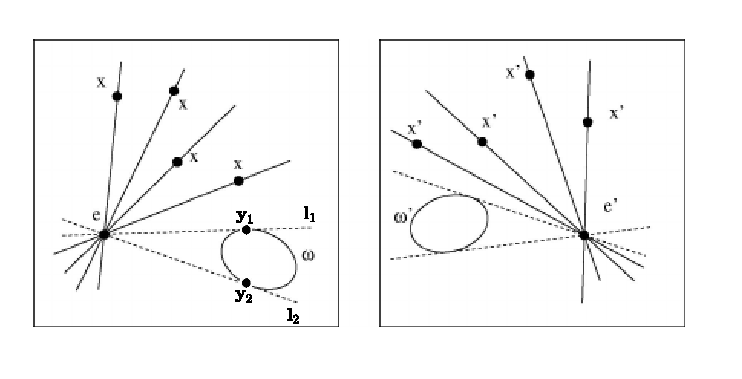
\includegraphics[scale=1]{restricao-epipolar-kruppa}
\caption{\textit{Retas epipolares tangentes às cônicas ${\bf \omega}$ e ${\bf \omega'}$.}}
\label{epipolar-kruppa}
\end{figure}

A restrição Kruppa foi originalmente introduzida por \cite{faugeras92} e está relacionada com uma cônica contida num plano no espaco 3D e suas imagens nas duas câmeras, e é válida para cônicas gerais, mas aqui no nosso caso vamos tratar especificamente da cônica absoluta $\Omega_\infty$ contida no plano infinito $\bpi_\infty$ no espaço, e as imagens da cônica absoluta (IAC) ${\bf \omega}$ e ${\bf \omega'}$.

\begin{teorema}
As duas tangentes à IAC $\omega$ passando pelo epipolo $\e$ estão relacionadas por uma homografia da reta epipolar às duas tangentes à IAC $\omega'$ passando pelo epipolo $\e'$.
\end{teorema}

\begin{proof}
 Sendo ${\bf \omega}^*$ e ${{\bf \omega}^*}'$ as respectivas cônicas duais (DIAC), considere um plano passando pelo centro das duas câmeras e tangenciando essa cônica $\Omega_\infty$ no espaço. Por construção, esse plano vai projetar uma reta epipolar em cada imagem onde cada reta será tangente às imagens ${\bf \omega}$ e ${\bf \omega'}$ da cônica $\Omega_\infty$, observado na figura \ref{geometria-kruppa}. E suponha ainda que $\lightrgb_1$ e $\lightrgb_2$ sejam as retas tangentes à cônica ${\bf \omega}$ na primeira imagem conforme a figura \ref{epipolar-kruppa}. Com essas duas retas tangentes podemos construir uma cônica degenerada $D$ (posto $2$) na forma  

\begin{equation}\label{eq.def.con.deg}
D=[\e]_\times\,{\bf \omega}^*\,[\e]_\times. 
\end{equation}

Para mostrar que $D$ é uma cônica (ponto) temos que verificar que é válida a relação $\y_1^\top D\,\y_1=0$, onde $\y_1\in\lightrgb_1$.

\begin{equation*}
\begin{array}{rcll}
\y_1^\top\,D\,\y_1&=&\y_1^\top [\e]_\times\,{\bf \omega}^*\,[\e]_\times\,\y_1&\\
&=&([\e]^\top_\times\,\y_1)^\top {\bf \omega}^*\,[\e]_\times\,\y_1&\\
&=&\lightrgb_1^\top {\bf \omega}^*\,\lightrgb_1& \qquad\text{pois}\qquad\lightrgb_1=\e\times\y_1\\
&=&0&
\end{array}
\end{equation*}
onde a última passagem segue do fato de ${\bf \omega}^*$ ser dual. Observe que usamos $[\e]^\top_\times\,\y_1=[\e]_\times\,\y_1$ quando na verdade $[\e]^\top_\times=-[\e]_\times$, mas aqui a diferença de escala é irrelevante. 

\begin{figure}[!htb]
\centering
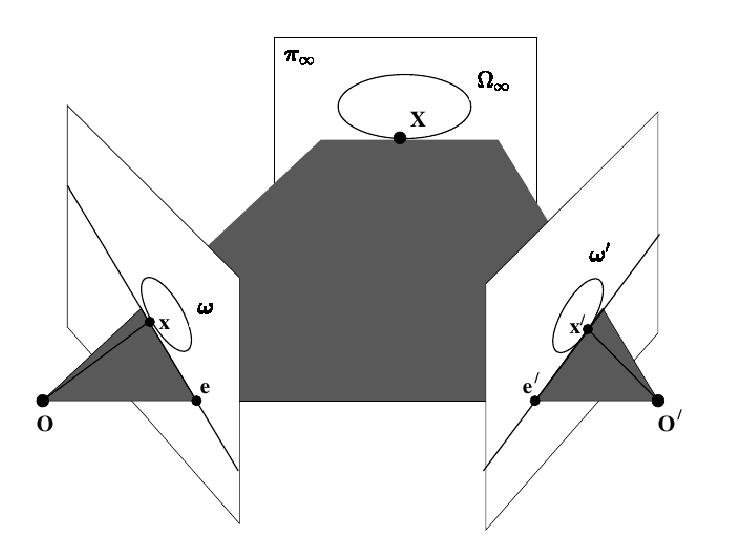
\includegraphics[scale=.9]{geometria-kruppa}
\caption{\textit{Um plano epipolar tangenciando uma cônica no espaco 3D projeta retas epipolares que tangenciam as cônicas nos planos das imagens}.}
\label{geometria-kruppa}
\end{figure}

Observamos que o desenvolvimento anterior é análogo para $\lightrgb_2$.

Na segunda imagem, analogamente à primeira, $D'=[\e']_\times\,{{\bf \omega}^*}'\,[\e']_\times$ e se transforma de acordo com a regra $D'=H_\infty^{-\top}D\,H_\infty^{-1}$ na subseção \ref{sec.trans-proj-H}. O símbolo $\infty$ se deve ao fato de que a homografia foi deduzida de maneria similar àquela da subseção  \ref{sec.homografia}, apenas com a diferença de ter sido com base no plano no infinito. Assim:

\begin{equation}\label{eq.kruppa}
\begin{array}{rcll}
[\e']_\times\,{{\bf \omega}^*}'\,[\e']_\times&=&D'&\\
&=&H_\infty^{-\top}D\,H_\infty^{-1}&\\
&=&H_\infty^{-\top}[\e]_\times\,{\bf \omega}^*\,[\e]_\times\,H_\infty^{-1}&\qquad\text{pois}\qquad D=[\e]_\times\,{\bf \omega}^*\,[\e]_\times\\
%&=&F\,\omega^* F^\top,&
\end{array}
\end{equation}
%onde $F=H_\infty^{-\top}\,[\e]_\times$ conforme a %subseção \ref{sec.matriz-F}. 
Como $\omega^*$ é uma cônica envelope, formada pelas retas que são tangentes à $\omega$, temos que essas tangentes estão projetivamente relacionadas, em conjunto, pela equação \ref{eq.kruppa}. Como as tangentes passam pelos epipolos, são retas epipolares e o teorema segue.

\end{proof}
Observe que, como conjunto, as tangentes não vêm em qualquer ordem particular, pois a relação não explicita uma mapeamento individual entre as retas, há apenas a relação entre produtos simétricos. Mas veremos na subseção \ref{sec.teorema-5} que esse fato não causará problemas.



\subsection{Mudança de coordenadas projetivas}

De acordo com \cite{kneebone}, podemos escolher as coordenadas projetivas de forma que os quatro pontos tenham as mesmas coordenadas em cada imagem. Ou seja, podemos assumir que ${\bf x}_i = {\bf x'}_i$ pensando nos dois planos de imagem como registrados no mesmo sistema de coordenadas. Vejamos como isso pode ser feito.

\subsubsection{Corregistro de pontos pertencentes a diferentes planos de imagem}\label{sec.corregistro-pontos}
Suponha a existência de pontos correspondência em dois planos de imagem relacionados por uma transformação projetiva $\x'=H\,\x$, onde $\x\in {\mathbb{P}^2}$ e $\x'\in {\mathbb{P'}^2}$. Nosso objetivo é fazer o corregistro de pontos da segunda imagem no sistema de coordenadas da primeira imagem, mas também poderíamos fazer o corregistro dos pontos das duas imagens para um terceiro plano projetivo qualquer. Fazendo as seguintes mudanças de coordenadas projetivas

\begin{equation}\label{eq.igualando-coordenadas}
\begin{array}{rcl}
\overline{\x}\,&=&I\,\x\\
\overline{\x}'&=&H^{-1}\x',
\end{array}
\end{equation}
temos que $\x=\overline{\x}$ e $\x'=H\,\overline{\x}'$. Substituindo essas duas últimas igualdades em $\x'=H\,\x$ temos

\begin{equation*}
\begin{array}{rcll}
\x'&=&H\,\x&\Rightarrow\\
H\,\overline{\x}'&=&H\,\overline{\x}&\Rightarrow\\
\overline{\x}'&=&H^{-1}H\,\overline{\x}&\Rightarrow\\
\overline{\x}'&=&\overline{\x}.&
\end{array}
\end{equation*}
Cabe ressaltar que as mudanças de coordenadas em \ref{eq.igualando-coordenadas} não altera nosso desenvolvimento, já que aqui nos interessa propriedades que são invariantes sob transformações projetivas, como tangências, interseções e raz\~ao cruzada. Portanto, onde foi utilizada a matriz identidade poderia ter sido usada qualquer outra homografia no caso de transferência dos pontos para um terceiro plano qualquer. A homografia $H$ é determinada a partir dos quatro pontos correspondentes supostos inicialmente pelo artigo.

\subsection{O teorema 3}\label{sec.teorema-3}

Aplicando as mudanças de coordenadas descritas na subsec\~ao \ref{sec.corregistro-pontos} nos quatro pontos e nos epipolos, temos que $\x=\x'$ e todos os seis pontos em questão estarão expressos no mesmo sistema de coordenadas, no mesmo plano de imagem. Observe a figura \ref{pontos-conconicos}.

\begin{teorema}
Os epipolos $\e$, $\e'$ e os quatro pontos $\x_i$ na imagem devem pertencer a uma cônica $B$. Reciprocamente, dois epipolos que são co-cônicos com os quatro pontos na imagem devem satisfazer à restricão epipolar.
\end{teorema}

\begin{proof}
Pela subseção \ref{sec.definicao-conica}, uma cônica fica determinada por cinco pontos, como temos quatro pontos na imagem vamos deixar a cônica $B$ na dependência de $\e$ (o quinto ponto necessário). Analogamente, o epipolo $\e'$ também define uma cônica com os quatro pontos na imagem, digamos $B'$. Pela subsec\~ao \ref{sec.homografia-reta-epipolar}, existe a homografia da reta epipolar que relaciona as quatro retas do feixe passando por $\e$ com as quatro retas do feixe passando por $\e'$. Pelo teorema de Steiner, \citep{kneebone}, se dois feixes de retas passando por $\e$ e $\e'$ estão homograficamente relacionados, o ponto de interseção entre retas correspondentes desses feixes descreve uma cônica que passa por $\e$ e $\e'$. Portanto $B=B'$ e todos os seis pontos em questão são co-cônicos.


Reciprocamente, pelo teorema de Chasles em \citep{kneebone}, se quatro pontos $\x_i$ numa cônica formam um feixe de retas concorrentes em um quinto ponto $\e\in B$, a razão cruzada entre as quatro retas não depende da posição de $\e$. Assim, a razão cruzada  do feixe concorrente em $\e$ é igual a do feixe concorrente em $\e'$. Pela subseção \ref{sec.geometria-1D}, a razão cruzada num feixe de retas é igual a razão cruzada entre os quatro pontos de interseção de uma reta qualquer com o feixe. Pelo corolário ainda na subseção \ref{sec.geometria-1D}, dois conjuntos de quatro pontos colineares têm a mesma razão cruzada se, e somente se, correspondem sob uma homografia.  Pela dualidade da representação entre pontos e retas, temos a homografia entre retas epipolares.  
\end{proof}

Esta cônica $B=B(\e)$ será bastante importante durante a abordagem pois, se os dois epipolos são co-cônicos com os quatro pontos na imagem, figura \ref{pontos-conconicos}, existe uma \textit{única} homografia de reta epipolar que faz a relação das retas através ${\bf e}$ com as retas através ${\bf e'}$. 

\begin{figure}[!htb]
\centering
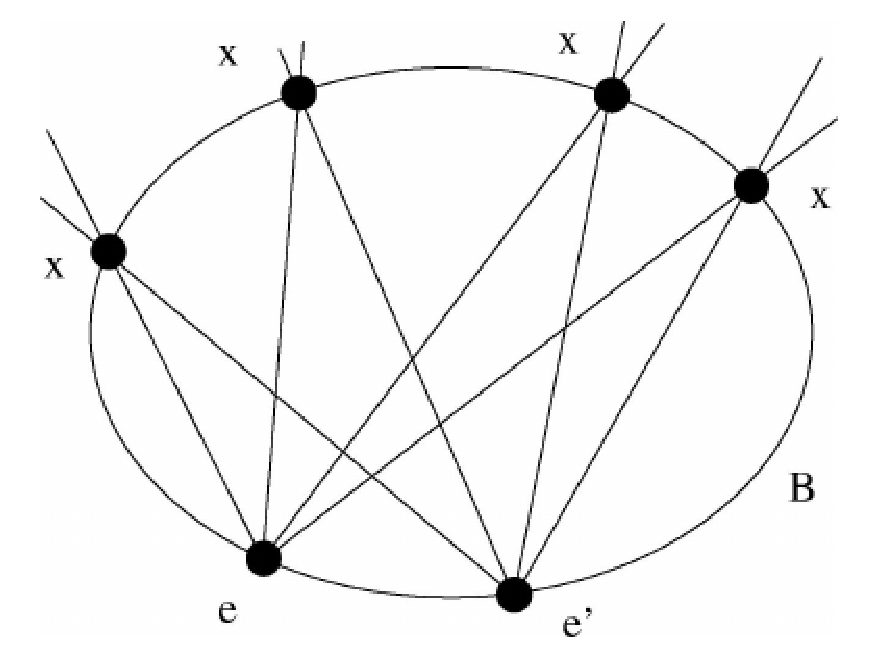
\includegraphics[scale=1.2]{pontos-conconicos}
\caption{\textit{Epipolos co-cônicos com os quatro pontos na imagem produzem homografia única.}}
\label{pontos-conconicos}
\end{figure}

\subsection{O teorema 4}\label{sec.demonstracao-teo-4}

Note que podemos parametrizar o feixe de retas passando por ${\bf e'}$ (ou ${\bf e}$) por pontos pertencentes à cônica $B$, pois retas correspondentes nos dois feixes intersectam $B$ no mesmo ponto. 

\begin{teorema}
As restrições de calibração são equivalentes à condição de que duas retas tangentes a $\omega$ que passam por $\e$ intersectam a cônica $B$ nos mesmos dois pontos adicionais que as duas retas tangentes a $\omega'$ passando por $\e'$.
\end{teorema}

\begin{proof}
Na subseção \ref{sec.teorema-2}, vimos que as duas retas tangentes à conica $\omega$ estão projetivamente relacionadas com as duas tangentes à cônica $\omega'$. Pelo teorema de Steiner, o ponto de interseção entre duas retas correspondentes, em dois feixes homograficamente relacionados, descrevem uma cônica. Assim, as retas tangentes à cônica $\omega$ se intersectam às retas tangentes à cônica $\omega'$ em dois pontos adicionais sobre a cônica $B$. 
\end{proof}

Isto é, as projeções de ${\bf \omega}$ e ${\bf \omega'}$ em $B$, através dos respectivos epipolos, devem coincidir. Essa construção geométrica pode ser visualizada na figura \ref{omega-B} e será a fundação para o resto da abordagem. 

\begin{figure}[!htb]
\centering
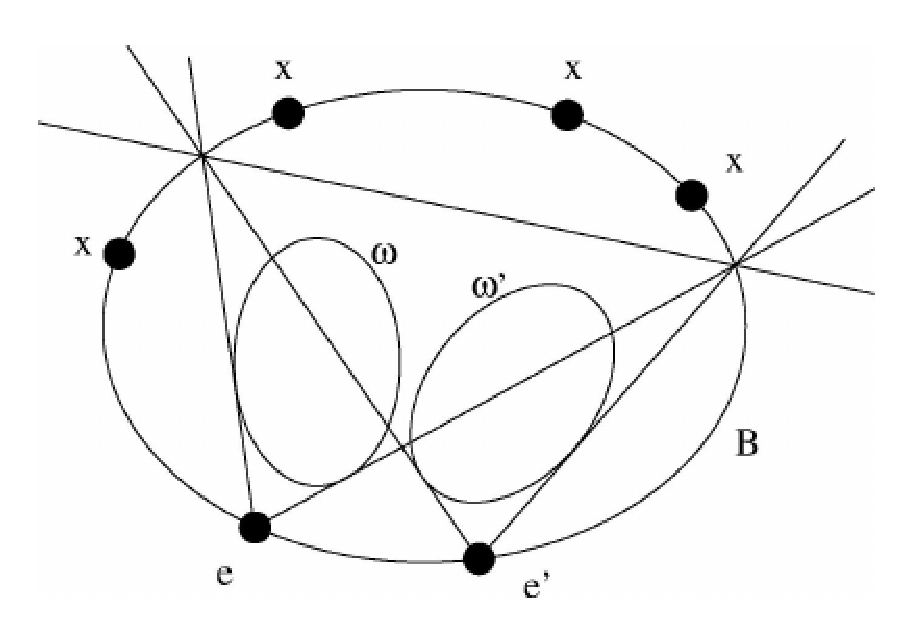
\includegraphics[scale=1.3]{projecao-omega-B}
\caption{\textit{Os pontos de interseção das tangentes com a cônica $B$ coincidem, ocasionando a coincidência das projeções das cônicas ${\bf \omega}$ e ${\bf \omega'}$ na cônica $B$.}}
\label{omega-B}
\end{figure}

\subsection{O teorema 5}\label{sec.teorema-5}

 A demonstração do próximo teorema é dada em \cite{2503343}, mas vamos incluir alguns detalhes e posteriormente dar uma demonstração extendida. Acompanhando pela figura \ref{omega-B}, podemos pensar na representação da projeção de  ${\bf \omega}$ e ${\bf \omega'}$ em $B$ como a reta que liga os dois pontos de interseção das tangentes com $B$, pois tal fato vai resolver o problema de que as tangentes não têm ordenação específica. Essa reta que liga os dois pontos de interseção, de acordo com a projeção de ${\bf \omega}$ através do epipolo ${\bf e}$ é representada por $({\bf \omega}\diamond B)\,{\bf e}$.

A equação \ref{eq.conica-diamond} é uma fórmula projetivamente invariante de uma cônica. Para ver isso, basta tomar a configuração para as cônicas $B$ e $\omega^*$ (mais a frente veremos o porquê dessas configurações)

\begin{equation*}
B=
\begin{bmatrix}
0&0&1\\
0&-2&0\\
1&0&0
\end{bmatrix}
\qquad\text{e}\qquad
\omega^*=
\begin{bmatrix}
c_{11}&c_{12}&c_{13}\\
c_{12}&c_{22}&c_{23}\\
c_{13}&c_{23}&c_{33}
\end{bmatrix},
\end{equation*} 
e efetuar as multiplicações constantes na equação \ref{eq.conica-diamond}. Lembrando que o traço de uma matriz é definido pela soma dos elementos da diagonal principal, o resultado das multiplicações é uma matriz simétrica, que pela subseção \ref{sec.definicao-conica}, representa uma cônica. Pela subseção \ref{sec.trans-proj-H}, uma homografia leva uma cônica em outra cônica, a qual mantém as características invariantes sob transformação projetiva.

\subsubsection{Representação canônica de uma cônica}\label{sec.forma-canonica-B}

Como vimos na subseção \ref{sec.espaco-P2}, o plano projetivo $\mathbb{P}^2$ tem seus pontos representados por vetores homogêneos com três componentes. Da Álgebra Linear sabemos que o espaço $\mathbb{R}^3$ também tem seus pontos representados por vetores com três componentes. Portanto, existe uma analogia entre as representações mesmo que no plano projetivo a relação entre vetores e pontos não seja biunívoca como em $\mathbb{R}^3$. Da mesma forma que podemos escolher a base canônica para representar vetores em $\mathbb{R}^3$, fazendo a devida transformação projetiva do sistema de coordeandas, podemos escolher uma base para representação do plano projetivo com a inclusão de um \textit{vetor unitário} ${\bf u}=(1,1,1)^\top$. Assim, cada ponto em $\mathbb{P}^2$ pode ser representado em termos da base \{$\x_1=(1,0,0)^\top,\x_2=(0,1,0)^\top,\x_3=(0,0,1)^\top,{\bf u}=(1,1,1)^\top$\} onde os três primeiros vetores são chamados {\it pontos de referência}. Para detalhes ver teorema 1 no apêndice  de \citep{kneebone}.

Os pontos de referência, que são linearmente independentes, formam os vértices de um triângulo chamado \textit{triângulo de referência}, com o ponto unitário no interior do triângulo. Esse triângulo vai servir como uma base para a representação do plano projetivo, conforme a figura \ref{fig.triangulo-referencia}. Por exemplo, representando um ponto qualquer por $\x=(x,y,z)^\top$ e uma reta qualquer por $\lightrgb=(a,b,c)^\top$ a reta determinada pelos pontos $\x_1$ e ${\bf u}$ tem equação $z-y=0$.

\begin{figure}[!htb]
\centering
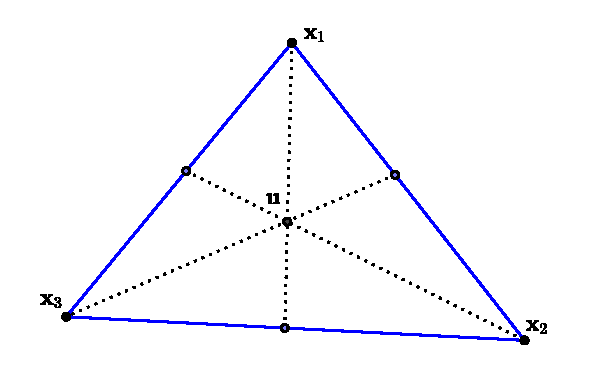
\includegraphics[scale=1]{triangulo-referencia}
\caption{{\it Triângulo de referência com vértices determinados por três vetores que, juntamente com o vetor unitário, servem de base para representação do plano projetivo.}}
\label{fig.triangulo-referencia}
\end{figure}

Pois, se $\x_1\in\lightrgb$ e ${\bf u}\in\lightrgb$ então

\begin{equation}\label{eq.exemplo-tri-referencia}
\lightrgb^\top{\bf u}=0\Rightarrow a+b+c=0\qquad\text{e}\qquad\lightrgb^\top\x_1=0\Rightarrow a=0.\qquad\text{Assim,}\quad b=-c.
\end{equation}

Dado um ponto qualquer $\x\in\lightrgb$ a equação da reta fica

\begin{equation*}
\lightrgb^\top\x=0\Rightarrow a\,x+b\,y+c\,z=0,
\end{equation*}
e usando as relações em \ref{eq.exemplo-tri-referencia} temos que

\begin{equation*}
-c\,y+c\,z=0\Rightarrow z-y=0,
\end{equation*}
já que $c\neq 0$ pois do contrário $\lightrgb$ representaria um ponto no infinito.

Existem algumas formas padronizadas pelas quais a representação da cônica $B$ pode ser simplificada através da escolha conveniente de uma estrutura de referência. Uma dessas escolhas é tomar o triângulo de referência como tendo dois de seus lados tangentes à cônica, e o terceiro lado como reta polar em relação ao seu vértice oposto, e escolher um ponto  da cônica como ponto unitário. Ver figura \ref{fig.conica-tri-referencia}.

\begin{figure}[!htb]
\centering
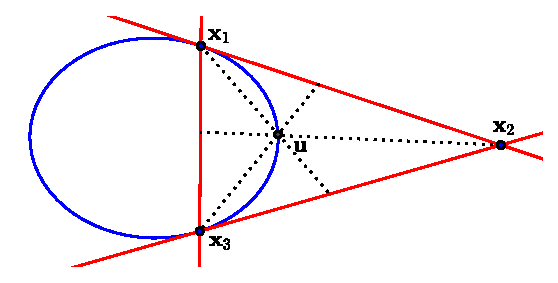
\includegraphics[scale=1]{conica-tri-referencia}
\caption{{\it A cônica $B$ numa relação polo-polar com um triângulo de referência que representa o plano projetivo $\mathbb{P}^2$}.}
\label{fig.conica-tri-referencia}
\end{figure}

Como vimos na subseção \ref{sec.definicao-conica}, a cônica $B$ pode ser representada na forma matricial com coordenadas homogêneas como

\begin{equation*}
\begin{pmatrix}
x&y&z
\end{pmatrix}
\begin{bmatrix}
a&b/2&c/2\\
b/2&d&e/2\\
c/2&e/2&f
\end{bmatrix}
\begin{pmatrix}
x\\
y\\
z
\end{pmatrix}
=0
\end{equation*}
ou através da equação

\begin{equation*}
a\,x^2+b\,x\,y+d\,y^2+c\,x\,z+e\,y\,z+f\,z^2=0.
\end{equation*}

Supondo que a cônica passe pelos pontos $\x_1=(1,0,0)^\top$ e $\x_3=(0,0,1)^\top$ temos que

\begin{equation*}
\x_1\in B\Rightarrow a=0\quad\text{e}\quad\x_3\in B\Rightarrow f=0,
\end{equation*}
daí a equação da cônica será 

\begin{equation}\label{eq.reducao-parcial-conica}
d\,y^2+b\,x\,y+c\,x\,z+e\,y\,z=0.
\end{equation}

Consirede a reta $\lightrgb=(l_1,l_2,l_3)^\top$ que passa pelos pontos $\x_1$ e $\x_3$,

\begin{equation*}
\lightrgb^\top\x_1=
\begin{pmatrix}
l_1&l_2&l_3
\end{pmatrix}
\begin{pmatrix}
1\\
0\\
0
\end{pmatrix}
=0
\Rightarrow l_1=0,
\end{equation*} 

\begin{equation*}
\lightrgb^\top\x_3=
\begin{pmatrix}
l_1&l_2&l_3
\end{pmatrix}
\begin{pmatrix}
0\\
0\\
1
\end{pmatrix}
=0
\Rightarrow l_3=0,
\end{equation*} 
e portanto $\lightrgb=(0,l_2,0)^\top$.

Observando que $\lightrgb$ está numa relação polo-polar com o ponto $\x_2$, pela subseção \ref{sec.polo-polar} temos que $B\,\x_2=\lightrgb$, daí

\begin{equation*}
\begin{bmatrix}
a&b/2&c/2\\
b/2&d&e/2\\
c/2&e/2&f
\end{bmatrix}
\begin{pmatrix}
0\\
1\\
0
\end{pmatrix}
=
\begin{pmatrix}
b/2\\
d\\
e/2
\end{pmatrix}
=
\begin{pmatrix}
0\\
l_2\\
0
\end{pmatrix},
\end{equation*}
e teremos $b=e=0$ e $d=l_2$.

Assim a equação \ref{eq.reducao-parcial-conica} toma a forma

\begin{equation}\label{eq.reducao-parcial2-conica}
l_2\,y^2+c\,x\,z=0,\quad\text{ou}\quad y^2=k\,x\,z\quad\text{com}\quad k=-\frac{c}{l_2}.
\end{equation}

A cônica $B$ passa também pelo ponto unitário ${\bf u}=(1,1,1)^\top$, assim substituindo na equação \ref{eq.reducao-parcial2-conica} temos que $k=1$, e a equação da cônica se reduz finalmente a 

\begin{equation}\label{eq.reducao-total-conica}
y^2=x\,z,
\end{equation}
que é a equação conônica da cônica em $\mathbb{P}^2$. Na forma matricial a cônica é representada por 

\begin{equation*}
B=
\begin{bmatrix}
0&0&1\\
0&-2&0\\
1&0&0
\end{bmatrix}.
\end{equation*}

\subsubsection{Representação canônica paramétrica}\label{sec.repre-canonica-parametrica}
A equação \ref{eq.reducao-total-conica} pode ser escrita na forma 

\begin{equation*}
\left(\frac{y}{z}\right)^2=\frac{x}{z},
\end{equation*}
e fazendo a substituição $\displaystyle{\frac{y}{z}=\theta}$ temos que $\displaystyle{\frac{x}{z}=\theta^2}$ e $x:y:z=\theta^2:\theta:1$.
Assim, todo ponto pertencente à cônica $B$ terá a forma $(\theta^2,\theta,1)^\top$, que é realmente uma parametrização da curva, no sentido de que existe uma relação biunívoca entre cada ponto da curva e o valor do parâmetro $\theta$. No caso do artigo de \citep{2503343} esta formalização é bastante útil pois, como a cônica $B$ está em função do quinto ponto, o epipolo $\e$, temos que esse ponto, e consequentemente a cônica, pode ser definida apenas pelo parâmetro $\theta$. Podemos observar que é válida a relação

\begin{equation*}
\begin{pmatrix}
1&\theta&\theta^2
\end{pmatrix}
\begin{bmatrix}
0&0&1\\
0&-2&0\\
1&0&0
\end{bmatrix}
\begin{pmatrix}
1\\
\theta\\
\theta^2
\end{pmatrix}
=0.
\end{equation*}


\subsubsection{Demonstração do teorema}

Após a apresentação dos conceitos necessários, vamos estabelecer o teorema e demonstrá-lo.

\begin{teorema}
A projeção da IAC $\omega$ na cônica $B$, usando o epipolo $\e$ como centro de projeção, é dada pelo ponto de interseção entre a reta $(\omega\diamond B)\,\e$ e $B$, onde a cônica $(\omega\diamond B)$ é definida como

\begin{equation}\label{eq.conica-diamond}
(\omega \diamond B)\equiv 2\,B\,\omega^*B - tr(\omega^*\,B)\,B.
\end{equation}
\end{teorema}

\begin{proof}

Pela subseção \ref{sec.demonstracao-teo-4}, a reta epipolar $\lightrgb$ tangente à IAC intersecta a cônica $B$ em um ponto ${\bf q}$, conforme a figura \ref{omega-B}. Como ${\bf q}\in B$ e $B$ tem a forma definida na subseção \ref{sec.forma-canonica-B}, temos que ${\bf q}$ pode ser parametrizado por ${\bf q}=(1,\lambda,\lambda^2)^\top$, conforme a subseção \ref{sec.repre-canonica-parametrica}. Desta forma, precisamos mostrar que ${\bf q}\in (\omega\diamond B)\,\e$, ou seja, $[(\omega\diamond B)\,\e]^\top {\bf q}=0$ onde $\e=(1,\theta,\theta^2)^\top$. A reta $\lightrgb$ pode ser definida pelos pontos $\e$ e ${\bf q}$ como $\lightrgb=\e\times {\bf q}$ e, fazendo as substituições, vem

\begin{equation*}
\begin{array}{rcl}
\lightrgb&=&(1,\theta ,\theta^2)\times (1,\lambda,\lambda^2)\\
&=&(\lambda -\theta)(\theta\lambda,-(\theta+\lambda),1)\\
&=&(\theta\lambda,-(\theta+\lambda),1)
\end{array}
\end{equation*}
ignorando o fator de escala $(\lambda-\theta)$.

Como $\lightrgb$ é tangente à cônica $\omega$, temos que a reta satisfaz a relação definida na subseção \ref{sec.conica-dual}, $\lightrgb^\top\omega^*\lightrgb=0$. Parametrizando $\omega^*$ por $[c_{ij}]$ temos que a relação $\lightrgb^\top\omega^*\lightrgb=0$ se torna

\begin{equation*}
\begin{pmatrix}
\theta\lambda&-(\theta+\lambda)&1
\end{pmatrix}
\begin{bmatrix}
c_{11}&c_{12}&c_{13}\\
c_{12}&c_{22}&c_{23}\\
c_{13}&c_{23}&c_{33}
\end{bmatrix}
\begin{pmatrix}
\theta\lambda\\
-(\theta+\lambda)\\
1
\end{pmatrix}
=0,
\end{equation*}  
que é equivalente à equação

\begin{equation}\label{eq.expandida-omega-dual}
\theta^2\lambda^2 c_{11}+(-2\,\theta^2\,\lambda-2\,\theta\lambda^2)\,c_{12}+2\,\theta\lambda\,c_{13}+(\theta+\lambda)^2\,c_{22}+(-2\,\theta-2\,\lambda)\,c_{23}+c_{33}=0.
\end{equation} 

Usando a definição de $(\omega\diamond B)$ em \ref{eq.conica-diamond}, a parametrização de $\omega^*$ por $[c_{ij}]$ e a forma canônica de $B$ (subseção \ref{sec.repre-canonica-parametrica}), temos que

\begin{equation*}
(\omega\diamond B)=
\begin{bmatrix}
2\,c_{33}&-4\,c_{23}&2\,c_{22}\\
-4\,c_{23}&4\,(c_{13}+c_{22})&-4\,c_{12}\\
2\,c_{22}&-4\,c_{12}&2\,c_{11}
\end{bmatrix},
\end{equation*}
e a relação $[(\omega\diamond B)\,\e]^\top {\bf q}=\e^\top (\omega\diamond B)\,{\bf q}=0$ se torna

\begin{equation*}
\begin{pmatrix}
1&\theta&\theta^2
\end{pmatrix}
\begin{bmatrix}
2\,c_{33}&-4\,c_{23}&2\,c_{22}\\
-4\,c_{23}&4\,(c_{13}+c_{22})&-4\,c_{12}\\
2\,c_{22}&-4\,c_{12}&2\,c_{11}
\end{bmatrix}
\begin{pmatrix}
1\\
\lambda\\
\lambda^2
\end{pmatrix}
=0,
\end{equation*}
que é equivalente à equação

\begin{equation}\label{eq.expandida-omega-diamond}
\theta^2\lambda^2 c_{11}+(-2\,\theta^2\,\lambda-2\,\theta\lambda^2)\,c_{12}+2\,\theta\lambda\,c_{13}+(\theta+\lambda)^2\,c_{22}+(-2\,\theta-2\,\lambda)\,c_{23}+c_{33}=0,
\end{equation}
a menos do fator de escala 2.

A equação \ref{eq.expandida-omega-dual} é igual à equação \ref{eq.expandida-omega-diamond}, e como 
\ref{eq.expandida-omega-dual} é uma relação válida, também é a equação \ref{eq.expandida-omega-diamond}. O teorema segue.
\end{proof}
Repare que o desenvolvimento é análogo para o segundo ponto de interseção da tangente à $\omega$ com $B$.


\subsection{O teorema 6}\label{sec.teorema-6}

\begin{teorema}
Dado que os epipolos $\e$ e $\e'$ são co-cônicos com quatro pontos na imagem, a restrição Kruppa é equivalente à restricao de que as retas $(\omega\diamond B)\,\e$ e $(\omega'\diamond B)\,\e'$ coincidem.
\end{teorema}

\begin{proof}
Pela subseção \ref{sec.demonstracao-teo-4}, a reta tangente à $\omega'$ intersecta $B$ nos mesmos pontos adicionais, onde um deles foi denotado por ${\bf q}$. Como os pontos são co-cônicos podemos usar a forma canônica de $B$ e a parametrização canônica para $\e'$. O desenvolvimento é análogo ao da subseção \ref{sec.teorema-5}.
\end{proof}

\subsection{O teorema 7}


Primeiramente note que $(\omega \diamond B) = B\,(\omega \cdot B)$ se definirmos a homografia

\begin{equation}
(\omega \cdot B) \equiv 2\,\omega^*\,B - tr(\omega^*\,B)\,I,
\end{equation}
onde está sendo ``cancelado" $B$ na definição de $(\omega \diamond B)$. Antes de passarmos ao teorema vamos fazer um esclarecimento sobre alguns conceitos. 

\subsubsection{Feixe de cônicas}\label{sec.feixe-conicas}

Dadas duas cônicas $B_1$ e $B_2$ pertencentes a $\mathbb{P}^2$, cujo a forma quadrática é definida por $\x^\top B_1\x=0$ e $\x^\top B_2\x=0$, chamamos de \textit{feixe de cônicas} a família de cônicas definidas por

\begin{equation}\label{eq.B-combinacao-B1-B2}
B=\lambda\,B_1+\mu\,B_2\quad\text{onde}\quad\x\in\mathbb{P}^2.
\end{equation}

Observe que as cônicas $B_1$ e $B_2$ também pertencem ao feixe, onde basta tomarmos os valores $\lambda=1$ e $\mu=0$ e vice-versa para verificarmos tal fato. Assim, quaisquer duas cônicas pertencentes ao feixe podem ser escolhidas como uma base para a representação do feixe. Resolvendo o sistema de equações

\begin{empheq}[left=\empheqlbrace]{align*}
\x^\top B_1\x&=0\\
\x^\top B_2\x&=0
\end{empheq}
temos vários casos para as soluções mas trataremos aqui somente do caso com quatro soluções distintas, já que \citep{2503343} pressupõe que sejam fornecidos quatro pontos em posições gerais no plano da imagem, os quais são utilizados na definição do feixe de cônicas.

Chamamos de {\it pontos base} de um feixe de cônicas, os pontos que são comuns a todas as cônicas do feixe, isto é, eles são os pontos de interseção das duas cônicas $B_1$ e $B_2$ que são a base do feixe. Assim, o feixe de cônicas fica definido pelos quatro pontos de interseção dessas duas cônicas.

Como os quatro pontos $\x_i$ que definem o feixe são todos diferentes, temos que o feixe contém exatamente três cônicas degeneradas que são constituídas por pares de retas. Definindo as retas por dois pontos temos um total de combinações de $C_{4,2}=6$ retas dadas por

\begin{equation*}
\lightrgb_k=\x_i\times\x_j\quad\text{com}\quad k=1,...,6,\,\,i=1,2,3,\,\,j=2,3,4,\quad\text{e}\quad i<j.
\end{equation*}
Pela subseção \ref{sec.conicas-degeneradas}, cada cônica degenerada do feixe pode ser expressa como

\begin{equation}
\begin{array}{rcl}
B_1&=&\lightrgb_1\lightrgb_2^\top+\lightrgb_2\lightrgb_1^\top\\
B_2&=&\lightrgb_3\lightrgb_4^\top+\lightrgb_4\lightrgb_3^\top\\
B_3&=&\lightrgb_5\lightrgb_6^\top+\lightrgb_6\lightrgb_5^\top.
\end{array}
\end{equation}
Observe que com seis retas temos uma total de combinações de $C_{6,2}=15$ cônicas, no entanto duas retas escolhidas devem passar pelos quatro pontos base, ou seja, duas retas não podem compartilhar um mesmo ponto base. Portanto temos apenas três cônicas degeneradas, as quais são normalmente usadas como base do feixe de cônicas por serem mais facilmente obtidas.
 
\subsubsection{Estabelecimento e demonstração do teorema}\label{sec.teorema-7}

O esquema para o próximo teorema está representado na figura \ref{inter-B-C} e o símbolo $\sim$ significa igualdade a menos da escala.

\begin{teorema}
Os epipolos estão ralacionados por 

\begin{equation}\label{eq.equiv-reta-polar-sem-B}
(\omega'\cdot B)\,\e'\sim (\omega\cdot B)\,\e\sim{\bf p}
\end{equation}
o que implica numa função de sétimo grau 

\begin{equation}\label{eq.map-7-grau}
{\bf e} \rightarrow {\bf e'} \sim (\omega' \cdot B)^*\,(\omega \cdot B)\,{\bf e}.
\end{equation}

A restrição Kruppa disponibiliza quatro soluções para o epipolo ${\bf e}$ na cônica $B$, e as soluções são as interseções  de $B$ com a curva 

\begin{equation}\label{eq.definicao-conica-C}
C \equiv (\omega \cdot B)^\top\,(\omega' \cdot B)^{*\,\top}\,B\,(\omega' \cdot B)^*(\omega \cdot B).
\end{equation}

\end{teorema}

\begin{proof}
Pela subseção \ref{sec.teorema-6} $(\omega\diamond B)\,\e\sim(\omega'\diamond B)\,\e'$, e como a cônica $B$ é própria (posto completo) podemos invertê-la e eliminá-la na definição de $(\omega\diamond B)$ e de $(\omega'\diamond B)$ para chegar à relação \ref{eq.equiv-reta-polar-sem-B}. Assumindo que $|(\omega'\cdot B)|\neq0$, podemos invertê-la e chegar na função em \ref{eq.map-7-grau}. Como $\e'\in B\Rightarrow \e'^\top B\,\e'=0$, e substituindo a função em \ref{eq.map-7-grau} vem

\begin{equation*}
\begin{array}{rcl}
0&=&\e'^\top B\,\e'\\
&=&((\omega' \cdot B)^*\,(\omega \cdot B)\,{\bf e})^\top B\,(\omega' \cdot B)^*\,(\omega \cdot B)\,{\bf e}\\
&=&\e^\top (\omega \cdot B)^\top (\omega' \cdot B)^{*\top}B\,(\omega' \cdot B)^*\,(\omega \cdot B)\,\e\\
&=&\e^\top C\,\e.
\end{array}
\end{equation*}  
Como $\e \in C$ e $\e\in B$, então $\e$ está na interseção entre as duas curvas.


\begin{figure}[!htb]
\centering
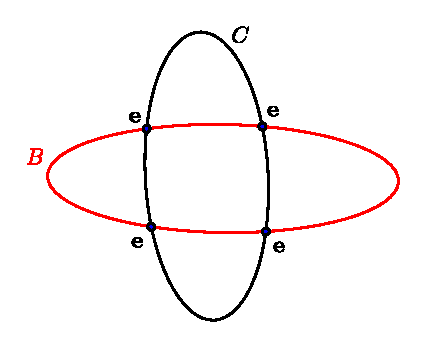
\includegraphics[scale=1]{intersecao-C-B}
\caption{\textit{Epipolos que satisfazem as restrições de projeção e de calibração podem ser encontrados como as interseções da cônica B com a curva C.}}
\label{inter-B-C}
\end{figure}

No caso em que $|(\omega'\cdot B)|=0$, devemos observar que, para câmeras e pontos em posições gerais (que excluem degenerações por serem casos raros), não há motivos para que $(\omega\cdot B)$ e $(\omega'\cdot B)$ se degenerem ao mesmo tempo. Assim, sendo $|(\omega'\cdot B)|=0$ podemos reescrever as equações \ref{eq.map-7-grau} e \ref{eq.definicao-conica-C} nas formas

\begin{equation*}
\e\sim (\omega\cdot B)^*(\omega'\cdot B)\,\e'\quad\text{e}\quad C_1 \equiv (\omega' \cdot B)^\top (\omega \cdot B)^{*\top}\,B\,(\omega \cdot B)^*\,(\omega' \cdot B).
\end{equation*}     
Analogamente à dedução anterior, $\e'\in C_1$ e a interseção de $B$ e $C_1$ vai gerar quatro soluções distintas para $\e'$.
 
 Podemos perceber, pela equação \ref{eq.map-7-grau}, a relação polo-polar entre o ponto ${\bf p}\sim (\omega'\cdot B)\,\e'$ e a reta $\lightrgb$ dada por $\lightrgb=B\,(\omega'\cdot B)\,\e'$ ou $\lightrgb=B\,{\bf p}$.
 % Assim, se ${\e'}\in B$ é uma das quatro soluções, existe uma outra solução para ${\e'}$ que vai gerar o mesmo ${\bf p}$, que vai ser a outra interseção da reta polar $\lightrgb$ com a cônica $B$. Desta forma, as soluções para ${\e'}$ se agrupam em dois pares.
 
 
Vimos que ${\bf p}\sim (\omega\cdot B)\,\e$ e, considerando novamente a curva 
\begin{equation*}
C \equiv (\omega \cdot B)^\top\,(\omega' \cdot B)^{*\,\top}\,B\,(\omega' \cdot B)^*(\omega \cdot B)
\end{equation*}                                      
temos, mesmo com  $|(\omega' \cdot B)|=0$, que
\begin{equation*}
\e^\top C\,\e=0\quad\text{ou}\quad
\e^\top (\omega \cdot B)^\top\,(\omega' \cdot B)^{*\,\top}\,B\,(\omega' \cdot B)^*(\omega \cdot B)\e=0,
\end{equation*}                                                pois
\begin{equation*}
\begin{array}{rcl}
(\omega' \cdot B)^*(\omega \cdot B)\e&\sim &(\omega' \cdot B)^*{\bf p}\\
&\sim &(\omega' \cdot B)^*(\omega'\cdot B)\,\e'\\
&\sim&|(\omega' \cdot B)|\,I\,\e'\\
&\sim&0\,I\,\e'\\
&\sim&{\bf 0}.
\end{array}
\end{equation*}
Assim, mesmo sendo $(\omega' \cdot B)$ degenerada temos que $\e\in C$.                                   
\end{proof}

Pela subseção \ref{sec.feixe-conicas}, temos que quaisquer duas cônicas de um feixe de côncias podem ser usadas como base do feixe, assim a cônica $B(\e)$ pode ser expressa na forma

\begin{equation*}
B(\e)=(\e^\top B_2\e)\,B_1-(\e^\top B_1\e)\,B_2,
\end{equation*} 
onde $B$ está sendo expressa em termos de $\e$, usando as cônicas $B_1$ e $B_2$ como base do feixe. Repare que os escalares $\e^\top B_2\e$ e $\e^\top B_1\e$ são sempre diferentes de zero pois, dados os quatro pontos $\x_i$ na imagem, a cônica $B$ fica unicamente determinada pelo quinto ponto $\e$, e portanto $\e\notin B_1$ e $\e\notin B_2$.


\subsection{O teorema 8}
Como a cônica $B$ está sendo expressa em termos de $\e$, para qualquer escolha de $\e$ teremos que $\e^\top B\,\e=0$, mas esse não é o caso para a curva $C$ definida na subseção \ref{sec.teorema-7}, e assim temos o próximo teorema.

\begin{teorema} 
Um epipolo hipotético $\e$ que define uma cônica $B$ satisfaz a equação de $16^{\underline{o}}$ grau 
\begin{equation}\label{eq.dezesseis}
\e^\top C\,\e=0
\end{equation}
se, e somente se, satisfaz as restrições de projetividade e calibração.
\end{teorema}
\begin{proof}
Esse teorema é uma consequência do teorema na subseção \ref{sec.teorema-7} onde vimos que os epipolos estão na interseção da cônica $B$ com a curva $C$, e portanto devem satisfazer a equação \ref{eq.dezesseis}. O teorema da subseção \ref{sec.teorema-7} é dependente da restrição de calibração na subseção \ref{sec.demonstracao-teo-4} e da restrição de projeção na subseção \ref{sec.teorema-5}. 
\end{proof}

\subsection{Teoremas 9,\,10 e 11}
Esses teoremas têm demonstração completa no artigo e não necessitam de consulta em bibliografia extra, apesar de conterem bastante desenvolvimento algébrico. A utilidade deles se resume em verificar que os possíveis epipolos pertencem à curva de equação $\e^\top C\,\e=0$ mesmo no caso onde $B(\e)$ é uma cônica degenerada, ou seja, a equação $\e^\top C\,\e=0$ contém $|B|$ como fator.   Nesse caso, os epipolos pertencem às seis retas que passam pelos quatro pontos $\x_i$ na imagem. Em seguida, é demonstrado como o fator $|B|$ pode ser eliminado da equação de $16^{\underline{o}}$ grau $\e^\top C\,\e=0$ para se chegar numa equação de $10^{\underline{o}}$ grau definida por
\begin{equation}
e^\top\,G\,e=0,
\label{dez}
\end{equation}
onde a curva $G$ é dada por
\begin{equation}
G=4\,U^\top D'^*\,B^*\,D'^*\,U-4\,t'^2\,B\,D\,D'^*\,(D\,B-t\,I)+s\,D^*-t^2\,t'^2\,D'^*,
\label{conica-G}
\end{equation}
com as definições:
\begin{equation*}
\begin{array}{rcl}
D&\equiv&\omega^*,\\
t&\equiv&tr(D\,B),\\
U&\equiv&(\omega \cdot B)\,\,\, \text{e}\\
s&=&(16\,|B|\,|D'|\,t'+t'^4-4\,t'^2\,tr(B^*\,D'^*)).
\end{array}
\end{equation*}
Na figura \ref{plot-C} podemos visualizar dois exemplos de curvas. À esquerda, uma curva com as seis retas passando pelos quatro pontos na imagem, definida pela equação \ref{eq.dezesseis} de $16^{\underline{o}}$ grau que contém $|B|$ como fator. À direita, a mesma curva sem as seis retas, depois de removido o fator $|B|$, definida pela equação \ref{dez} de $10^{\underline{o}}$ grau.   

\begin{figure}[!htb]
\centering
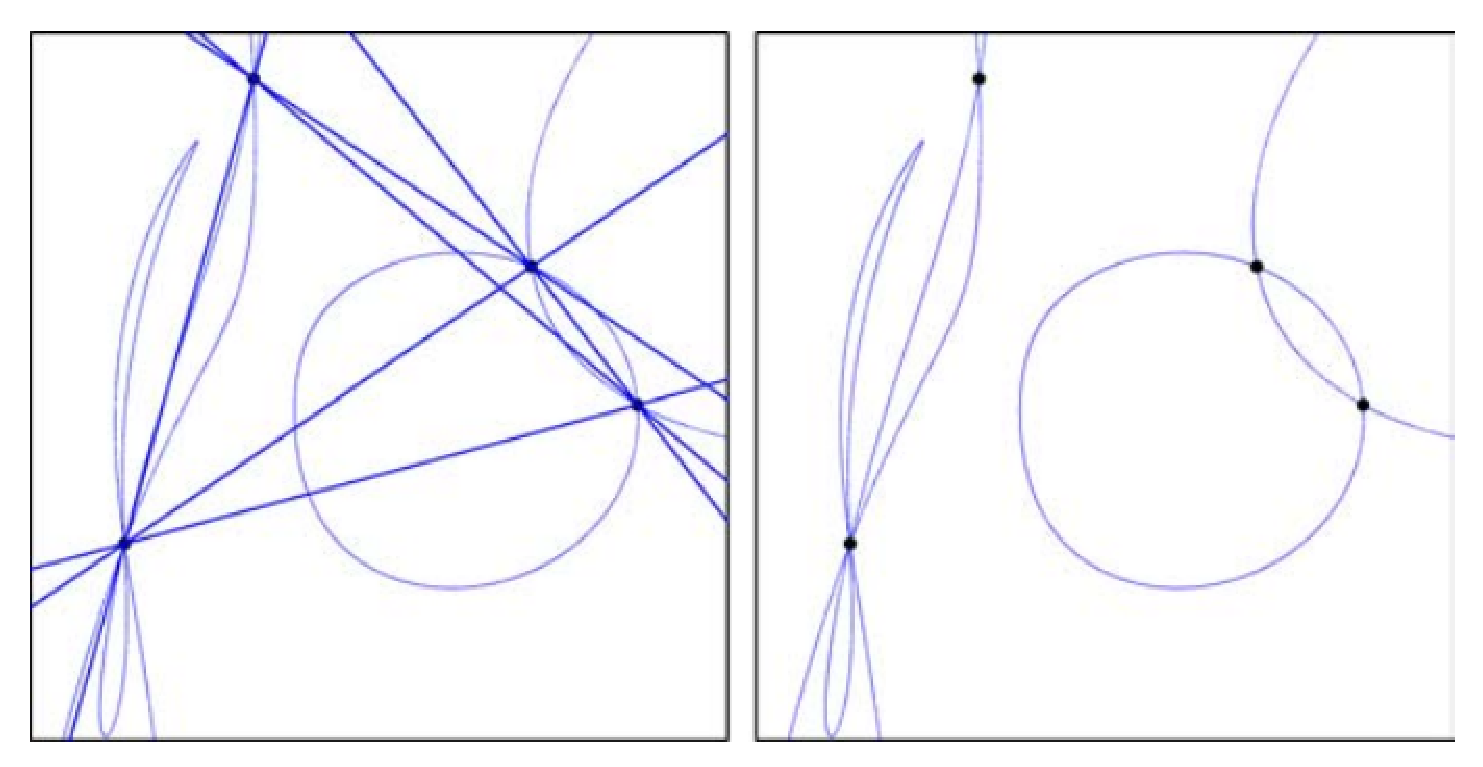
\includegraphics[scale=.4]{plotagem-C}
\caption{\textit{Podemos observar, à direita, a curva dos possíveis epipolos definida pela equação de décimo grau. À esquerda, a mesma curva com as seis retas, antes de removido o fator $|B|$ da equação de décimo-sexto grau.}}
\label{plot-C}
\end{figure}

\subsection{Teorema 12}
\begin{teorema}
Dados três pontos correspondentes e o epipolo $\e$
em uma imagem, as restrições de projeção e calibração possibilitam quatro soluções para o epipolo $\e'$ na outra imagem.
\end{teorema}
A demonstração desse teorema é construtiva e se trata de um algoritmo fornecido no apêndice do artigo. Temos quatro possibilidades para o epipolo $\e$ obtido como interseção da cônica $B$ com a curva de $10^{\underline{o}}$ grau $G$. E para cada um deles, temos quatro possibilidades para o epipolo $\e'$ de acordo com o algoritmo publicado no apêndice do artigo. Ou seja, como necessitamos dos pares de epipolos para obter a matriz esencial $E$, teremos um total de 16 possibilidades para $E$ para cada cônica $B$ do feixe de cônicas passando pelos quatro pontos na imagem dados inicialmente. 


\subsection{Teoremas 13 a 17}
Os teoremas 13 a 17 argumentam que a curva de grau 10 é exatamente a curva dos possíveis epipolos, e servem de base para o estabelecimento do principal resultado do artigo. Esses teoremas também possuem suas demonstrações no artigo.  

\subsection{Teorema 18}
É o principal resultado do artigo e sua demonstração é uma consequência dos teoremas 7, 10 e 17. O teorema é colocado como segue.

\begin{teorema}
Um ponto é um possivel epipolo de acordo com as restrições de projetividade e calibração se, e somente se, o ponto pertence à curva de grau 10 definida pela equação $e^\top\,G\,e=0$ conforme \ref{dez}. Para pontos $\e$ em geral pertencentes a essa curva, o outro epipolo $\e'$ pode ser calculado usando a função de sétimo grau, ${\bf e} \rightarrow {\bf e'} \sim (\omega' \cdot B)^*\,(\omega \cdot B)\,{\bf e}
$, dada em \ref{eq.map-7-grau}.
\end{teorema}

Na figura \ref{curva-10} observamos alguns exemplos de curvas de décimo grau com seus possíveis epipolos. 

\begin{figure}[!htb]
\centering
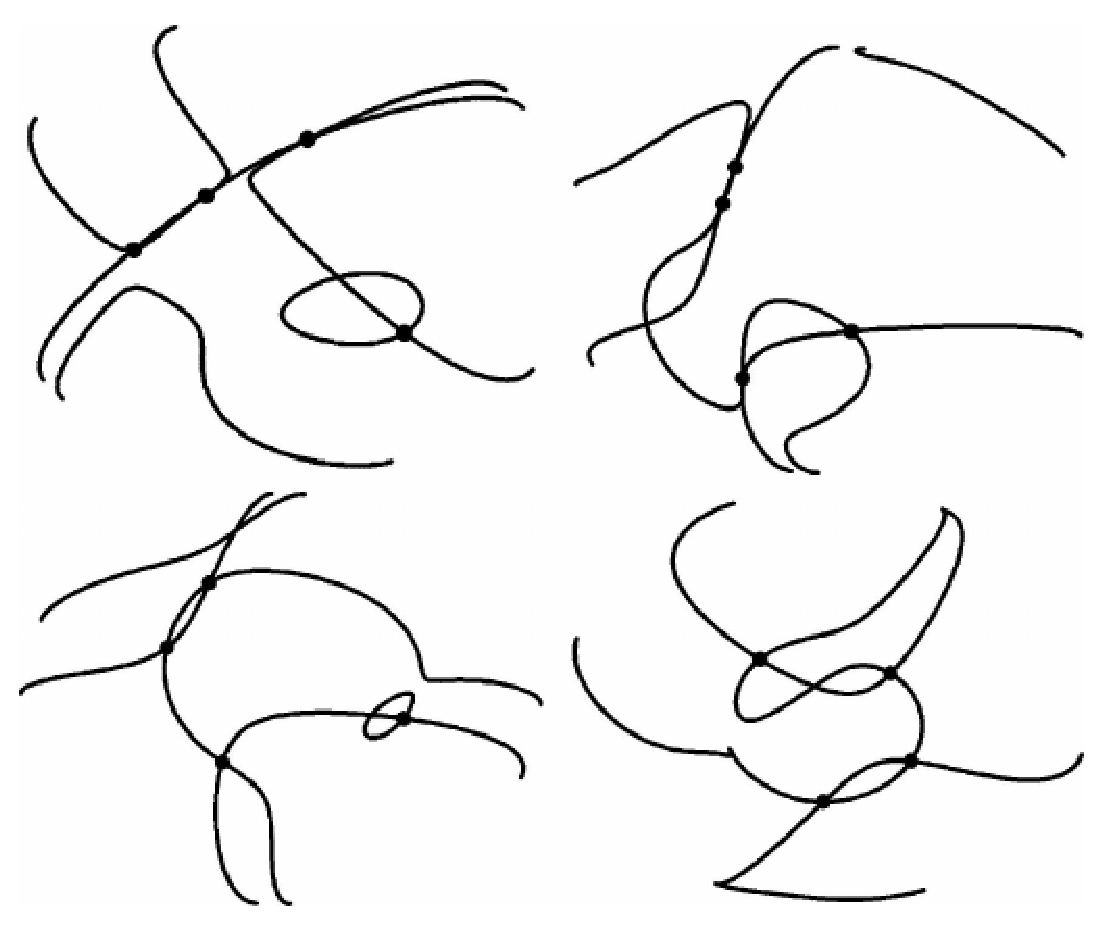
\includegraphics[scale=.4]{ex-curva-10}
\caption{\textit{Quatro exemplos de curvas de décimo grau definidas pela equação \ref{dez}, juntamente com seus respectivos epipolos.}}
\label{curva-10}
\end{figure}

\subsection{Teoremas 19 e 20}

Os teoremas 19 e 20 fornecem mais propriedades da curva de grau dez. O teorema 19 é uma versão mais completa do teorema 7 que se aplica mesmo quando a cônica $B$, definida em \ref{eq.B-combinacao-B1-B2}, é degenerada.

\subsection{Teoremas 21 a 25}

Esses teoremas tratam das restrições de orientação, para duas câmeras, e se resumem em dois fatos que podem ser visualizados na figura \ref{fig.quatro-essencial}. Primeiro, a {\it restrição de orientação epipolar}, onde as duas semirretas retroprojetadas por pontos correspondentes nas imagens devem estar no mesmo semiplano do plano epipolar (já que a reta base divide o plano epipolar em dois semiplanos). Ou seja, os pontos correspondentes devem estar alojados no mesmo semiplano. Segundo, a {\it restrição de convergência}, onde essas duas semirretas devem convergir para um ponto comum no espaço projetivo 3D.  

\subsubsection{A restrição de orientação}

Após determinados os epipolos, podemos determinar as retas epipolares através do produto vetorial entre os quatro pontos $\x_i$ e os epipolos. Com a retas epipolares podemos determinar a homografia da reta epipolar conforme a subseção \ref{sec.homografia-reta-epipolar}, para em seguida determinarmos a matriz essencial $E$ e a duas câmeras correspondentes. Mas existem quatro configurações para a determinação das duas câmeras, que são obtidas permutando a posição das duas câmeras (revertendo a orientação da reta base), ou rotacionando uma das câmeras $180^\circ$ em torno da reta base, ou os dois. As quatro configurações podem ser observadas na figura \ref{fig.quatro-essencial}. 
\begin{figure}[!htb]
\centering
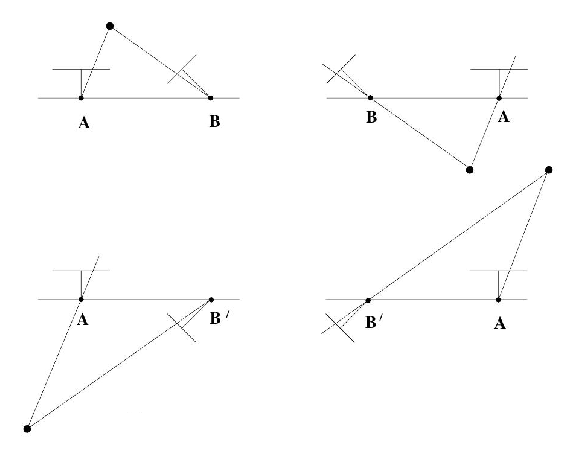
\includegraphics[scale=1]{quatro-configuracoes-essencial}
\caption{{\it Entre as imagens da direita e esquerda há a reversão da reta base. Entre as imagens de cima e de baixo há a rotação da câmera $180^\circ$ em torno da reta base. Apenas em uma das quatro configurações o ponto 3D está em frente as duas câmeras.}}
\label{fig.quatro-essencial}
\end{figure}
A restrição de orientação é exatamente o fato de o ponto 3D deve estar na parte da frente das duas câmeras. \citep{2503343} apresenta um método onde a restrição é satizfeita dependendo das posições relativas entre os epipolos fornecidos pela curva de grau 10 e os quatro pontos $\x_i$.

\subsubsection{A restrição de convergência}
Após a aplicação da restrição de orientação precisamos saber se as retas retroprojetadas pelos pontos correspondentes se intersectam em um ponto no plano epipolar. Tal interseção depende da relação entre o ângulo formado pelas retroprojeções de $\x_i$ e $\e$, e o ângulo formado pelas retroprojeções de $\x'_i$ e $\e'$. Um ponto 3D no sistema de coordenadas da câmera pode ser escrito como $\X=(\lambda {\bf d}^\top,1)^\top$, e é projetado na imagem através da equação de projeção
\begin{equation*}
\begin{array}{rcl}
\x&=&K[I|{\bf 0}]\X\\
\x&=&K[I|{\bf 0}](\lambda {\bf d}^\top,1)^\top\\
\x&=&K{\bf d}\quad\text{a menos da escala.}
\end{array}
\end{equation*}
O vetor ${\bf d}$ é a direção da reta retroprojetada por $\x$ e pode ser obtido pela expressão ${\bf d}=K^{-1}\x$, medido no sistema de coordenadas da câmera.
\begin{figure}[!htb]
\centering
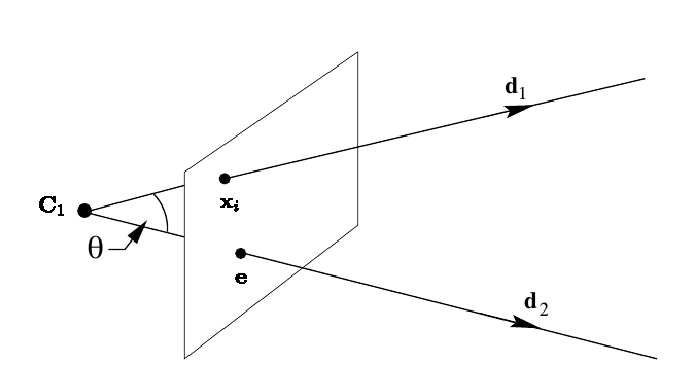
\includegraphics[scale=.8]{angulo-dois-pontos}
\caption{{\it O ângulo $\theta$ formado pelas retas retroprojetadas pelos pontos $\x_i$ e $\e$ através do centro de projeção ${\bf C}_1$ da primeira câmera. O procedimento é análogo para $\x'_i$ e $\e'$ na segunda câmera.}}
\end{figure}
Sabemos da Álgebra Linear que, dados dois vetores ${\bf d}_1$ e ${\bf d}_2$, a desigualdade de Cauchy-Schuarz é dada pela relação 
\begin{equation*}
|\left\langle{\bf d}_1,{\bf d}_2\right\rangle|\leq\left\|{\bf d}_1\right\|\left\|{\bf d}_2\right\|\quad\text{ou}\quad -1\leq\frac{\left\langle{\bf d}_1,{\bf d}_2\right\rangle}{\left\|{\bf d}_1\right\|\left\|{\bf d}_2\right\|}\leq 1,
\end{equation*}
onde, usando a multiplicação matricial podemos derivar uma relação para o cosseno do ângulo entre dois vetores
\begin{equation*}
\cos\theta=\frac{{\bf d}_1^\top{\bf d}_2}{\sqrt{{\bf d}_1^\top{\bf d}_1}\sqrt{{\bf d}_2^\top{\bf d}_2}},
\end{equation*}
com os vetores ${\bf d}_1=K^{-1}\x$ e ${\bf d}_2=K^{-1}\e$. Aplicando a substituição temos
\begin{equation*}
\cos\theta=\frac{(K^{-1}\x)^\top K^{-1}\e}{\sqrt{(K^{-1}\x)^\top K^{-1}\x}\sqrt{(K^{-1}\e)^\top K^{-1}\e}}
\end{equation*}
\begin{equation}\label{eq.cos-theta}
\cos\theta=\frac{\x^\top K^{-\top} K^{-1}\e}{\sqrt{\x^\top K^{-\top} K^{-1}\x}\sqrt{\e^\top K^{-\top} K^{-1}\e}}.
\end{equation}
Como \citep{2503343} supõe que a câmera é calibrada, ou seja, conhecemos a matriz $K$, podemos determinar o ângulo entre duas retas retroprojetadas por pontos no plano da imagem. Por isso, uma câmera calibrada é chamada {\it sensor de direção}.

Observe que, pela subseção \ref{sec.omega-calibracao}, podemos determinar a imagem da cônica absoluta IAC a partir da matriz de calibração, e a equação \ref{eq.cos-theta} se torna
\begin{equation}\label{eq.cos-omega}
\cos\theta=\frac{\x^\top\omega\,\e}{\sqrt{\x^\top\omega\,\x}\sqrt{\e^\top\omega\,\e}}.
\end{equation} 

O desenvolvimento é análogo para $\x'_i$ e $\e'$ escritos em outro sistema de coordenadas, pois a equação \ref{eq.cos-omega} é projetivamente invariante. De fato, considerando uma transformação projetiva $H$ onde, pela subseção \ref{sec.trans-proj-H},  $\x'=H\,\x$, a equação \ref{eq.cos-omega} fica
\begin{equation*}
\cos\theta=\frac{(H^{-1}\x')^\top\omega\,H^{-1}\e'}{\sqrt{(H^{-1}\x')^\top\omega\,H^{-1}\x'}\sqrt{(H^{-1}\e')^\top\omega\,H^{-1}\e'}}
\end{equation*} 
\begin{equation*}
\cos\theta=\frac{\x'^\top H^{-\top}\omega\,H^{-1}\e'}{\sqrt{\x'^\top H^{-\top}\omega\,H^{-1}\x'}\sqrt{\e'^\top H^{-\top}\omega\,H^{-1}\e'}}
\end{equation*}
\begin{equation*}
\cos\theta=\frac{\x'^\top \omega'\,\e'}{\sqrt{\x'^\top \omega'\,\x'}\sqrt{\e'^\top \omega'\,\e'}}
\end{equation*}
onde $\omega'=H^{-\top}\omega\,H^{-1}$ (como qualquer cônica se transforma) de acordo com a subseção \ref{sec.trans-proj-H}.

\subsection{Incluindo a terceira imagem}

As novidades do artigo se encontram na abordagem da reconstrução 3D para duas imagens e a aplicação a seguir segue o modelo padrão de projetar as reconstruções na terceira imagem e minimizar o erro em relação aos dados já disponíveis. Assim, dados quatro pontos numa imagem e suas respectivas correspondências em outras duas imagens (todas com as câmeras calibradas), podemos escolher duas dessas imagens para traçarmos a curva de décimo grau. Como vimos, temos quatro soluções para   ${\bf e}$ e cada solução pode ser usada para calcular ${\bf e'}$ na segunda imagem de acordo com a equação \ref{eq.map-7-grau}. Com os epipolos encontramos a homografia da reta epipolar  e daí, a matriz essencial relativa às duas imagens. Em seguida, podemos extrair as câmeras e usá-las para reconstrução dos pontos 3D a partir da triangulação usando duas imagens. Três pontos 3D juntamente com suas projeções (já conhecidas) são suficientes para determinar a câmera da terceira imagem, e podemos usar o quarto ponto para ser projetado na terceira imagem e comparar a projeção com o dado já obtido para refinar o resultado. Ou seja, o procedimento consiste em minimizar um erro na imagem. Como o problema é supra restringido por um grau de liberdade, com os ruídos das correspondências, o valores encontrados para a reprojeção do quarto ponto não coincidirá com o dado observado mesmo que usada a correta solução. Como para cada $\theta$ escolhido teremos dezesseis configurações de câmera da terceria imagem e dezesseis reprojeções, todas essas reprojeções definem uma complexidade enorme de curvas na terceira imagem. Na figura \ref{curvas-f(theta)} é dada uma ideia da dificuldade extrema do problema envolvendo três imagens e quatro pontos. 

\begin{figure}[!htb]
\centering
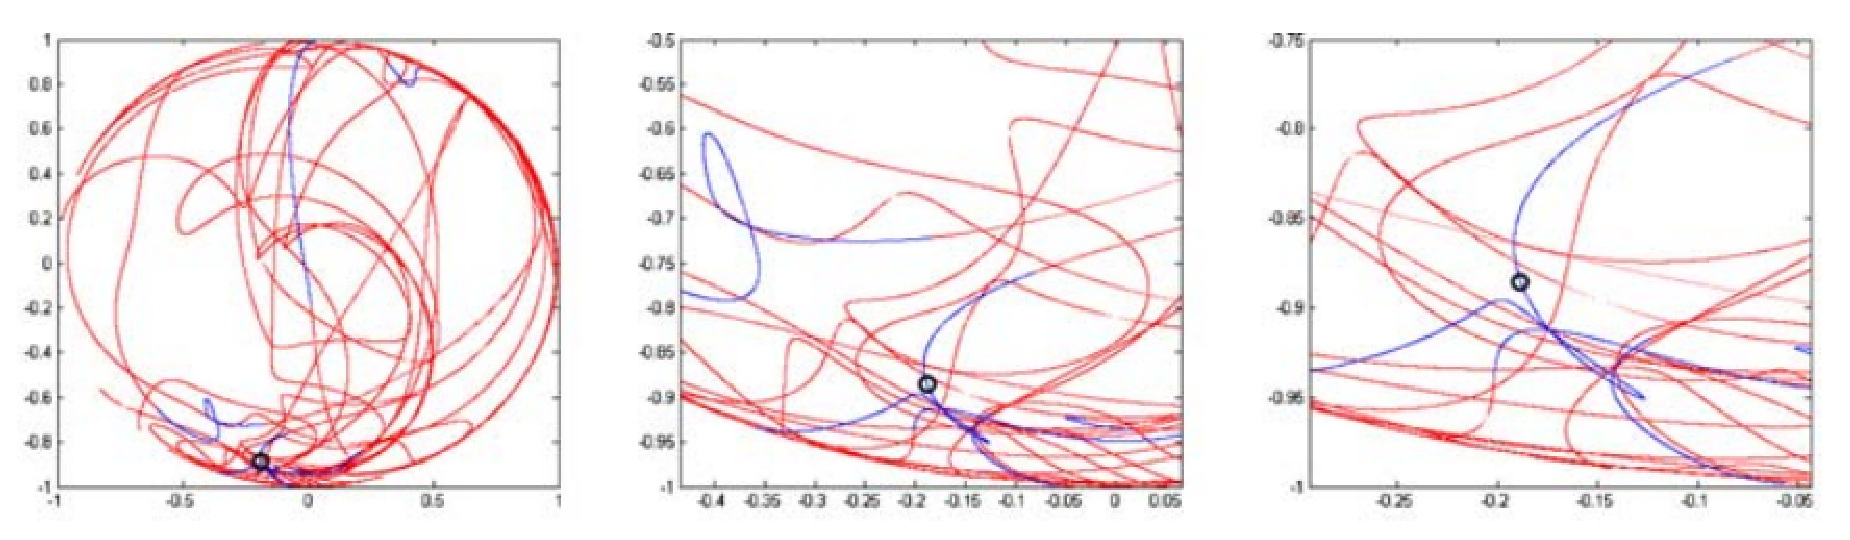
\includegraphics[scale=.52]{varias-curvas-f-theta}
\caption{\textit{A reprojeção do feixe de cônicas na terceira imagem e do quarto ponto reconstruído nos dá uma ideia da dificuldade do problema de três imagens com quatro pontos.}}
\label{curvas-f(theta)}
\end{figure}
